\documentclass[a4paper,openany,12pt]{book}
\usepackage{graphicx}
\usepackage[spanish]{babel}
\usepackage[utf8]{inputenc}
\usepackage{fancyhdr}
\usepackage{ae}
\usepackage[left=2.5cm,right=2.5cm,top=3cm,bottom=3cm]{geometry}
\usepackage[printonlyused]{acronym}
\usepackage{hlundef}
\usepackage{tesis}

\title{Título de la Tesis}

\author{Nombre completo del Autor de la Tesis}

\orientador{Prof Dr./Mag./Ing. Nombre del Asesor}

\dedicado{Aquí deberás colocar a
quien va dedicada tu tesis por ejemplo: A Dios, por todo lo que me
ha dado, a todos los profesores por sus enseñanzas y algunos
amigos.}

\begin{document}

\maketitle 

%Compone la carátula y la dedicatoria

%mayores detalles de como usas las abreviaturas (acronimos)
% vea: http://www.ctan.org/tex-archive/macros/latex/contrib/acronym/
% hay un manual en pdf en esa misma direccion

\chapter*{Abreviaturas}

\begin{acronym}
\acro{SPC}{Sociedad Peruana de Computación}
\acro{CMM}{\textit{Capability Maturity Model}}
\end{acronym}

\begin{agradecimientos}
Aquí deberás colocar a quien y porque agradeces. Ejemplo:

En primer lugar deseo agradecer a Dios por haberme guiado a lo largo de estos cinco años de estudio.

Agradezco a mis padres por el apoyo brindado para forjarme como un profesional.

Agradezco a la universidad, mi \textit{alma matter}, por haberme cobijado y brindado la formación que ahora me permitirá ayudar a construir una mejor sociedad.

Agradezco de forma muy especial a mi orientador Prof. Dr./Mag. nombre 1 por haberme guiado en esta tesis. ...

Deseo agradecer de forma especial a mis docentes: nombre 1, nombre 2, nombre 3 porque fueron ejemplos que deseo seguir en mi vida profesional.

Deseo agradecer al personal administrativo de la universidad: nombre 1, nombre 2, nombre 3. Muchas gracias por la atención brindada y porque siempre estuvieron dispuestas a ayudarnos.
\end{agradecimientos}
 %Inserta los agradecimientos
\begin{resumen}
Aquí deberás colocar entre 100 y 150 palabras como
máximo, el problema que intentas resolver, la
justificación y los aportes o soluciones que planteas.
\end{resumen}
 %Inserta el resumen
\begin{abstract}
Here you must write between 100 and 150 words about your thesis. 

In this text you must highlight your main contributions to this field.
\end{abstract}
 %Inserta el abstract

\tableofcontents %Inserta el índice general
\listoftables %Inserta el índice de cuadros
\listoffigures %Inserta el índice de figuras

%%%%%%%%%%%%%%%%%%%%%%%%%%%%%%%%%%%%%%%%%%%%%%%%%%%%%%%%%%%%%%%%%%%%%
%%%%   En esta parte deberas incluir los archivos de tu tesis   %%%%%
%%%%%%%%%%%%%%%%%%%%%%%%%%%%%%%%%%%%%%%%%%%%%%%%%%%%%%%%%%%%%%%%%%%%%

\chapter{Introducción}

Este es el primer capítulo de la tesis. Se inicia con el desarrollo de la introducción de la tesis. Es importante que el texto utilice la tabla de abreviaturas correctamente. En el archivo abreviaturas.tex contiene la tabla de abreviaturas. Para citar alguna de ellas debes usar los comandos $\backslash$ac\{tu-sigla-aqui\}. Si es la primera vez que utilizas la sigla ella se expandirá por completo. Por ejemplo, el comando $\backslash$ac\{CMM\} va a producir: \ac{CMM}. Si más adelante repites el mismo comando sólo aparecerá la sigla \ac{CMM}. Para explorar mucho más este comando es necesario leer su manual disponible en: $http://www.ctan.org/tex-archive/macros/latex/contrib/acronym/$


\section{Motivación y Contexto}

En esta sección se va desde aspectos generales a  aspectos específicos (como un embudo). No se olvide que es la primera parte que tiene contacto con el lector y que hará que este se interese en el tema a investigar.

El objetivo de esta sección es llevar al lector hacie el tema que se va a tratar en forma específica y dejar la puerta abierta a otras investigaciones

\section{Planteamiento del Problema}

En esta sección se realiza el planteamiento del problema que queremos resolver con la tesis. Sea muy puntual y no ocupe más de un párrafo en especificar cual es el problema que desea atacar.

\section{Objetivos}

En esta sección se colocan los objetivos generales de la tesis. Máximo dos. Si necesita ampliar estos objetivos utilice la sección de objetivos específicos.

\subsection{Objetivos Específicos}

En esta sección se coloca el los objetivos específicos de la tesis, que serán aquellos que contesten a las
interrogantes de investigación.

\section{Organización de la tesis}

En esta sección se coloca cuantos capítulos contendrá la tesis y que se tratará en cada uno de
ellos en forma resumida. Dediquele un parrafo de dos o tres lineas a explicar cada capítulo.

 %Inserta el capítulo 1
\chapter{Trabajos Relacionados}
\section{Consideraciones Iniciales}
En este capítulo se discute... 
\section{Minería Visual de Datos}

Cuando se hace análisis de datos primero se especifica ciertos parámetros para restringir el espacio de búsqueda; de esta forma la minería de datos trabaja de forma automática siguiendo un algoritmo (matemático, estadístico o de inteligencia artificial), finalmente los patrones son encontrados por este algoritmo para luego ser presentados como resultados en pantalla. Dado que existe gran cantidad de patrones generados por el algoritmo de minería de datos automática en forma textual, es casi imposible para el ser humano interpretar y evaluar el patrón en detalle para extraer conocimientos interesantes y características generales. Por otra parte la visualización de información es un estudio de representaciones (interactivas) visuales de datos para reforzar la cognición humana. Estas dos estrategias de de tratamiento de información (minería de datos y visualización de información) pueden llegar a ser complementarias y coexistir en la búsqueda de soluciones para la interpretación de un conjunto de datos complejos o naturales. Por lo tanto, para que la minería de datos sea efectiva es importante incluir a los humanos en el proceso de exploración de datos y combinar la flexibilidad, creatividad y el conocimiento general de la persona con la gran capacidad de almacenamiento y procesamiento de las computadoras de hoy en día. Tal área es denominada \textit{Minería Visual de Datos} \cite{wong1999guest}.

La minería visual de datos tiene como objetivo la integración del humano en el proceso de minería de datos, y la aplicación de las capacidades perceptivas de los humanos para el análisis de grandes conjuntos disponibles. la presentación de los datos en un formulario gráfico en interactivo a menudo fomenta la formación y la validación de nuevas hipótesis, para una buena toma de decisiones por consiguiente una buena resolución de los problemas. Con la visualización obtenemos una la formación y visión de estas hipótesis, la verificación de estas hipótesis se puede realizar también mediante la vía de visualización, pero lo mas conveniente es que vaya respaldado con algunas técnicas automáticas de análisis matemático, estadístico o aprendizaje maquina. 

Ankerst \cite{ankerst2001visual} clasifica en tres enfoques comunes la integración del humano en el proceso de exploración de datos como se muestra en la figura \ref{fig:VDM} :
\begin{itemize}
	\item \textbf{Visualización Anterior.} La visualización de información se realiza antes de que el algoritmo de minería de datos sea ejecutado, con la interacción se tiene un control total sobre el espacio de búsqueda. 
	\item \textbf{Visualización Posterior.} El algoritmo de minería de datos automática se ejecuta primero para la extracción de patrones y estos son mostrados por la visualización, se puede hacer re-calibraciones para posteriores exploraciones, esto con el objetivo de introducir otros parámetros y obtener mejores resultados.
	\item \textbf{Visualización fuertemente Integrado.} Un algoritmo de minería de datos automática realiza un análisis de los datos, pero no produce los resultados finales. Una técnica de visualización se utiliza para presentar los resultados  del proceso de exploración de datos. La combinación de algunos algoritmos de minería de datos automáticos y técnicas de visualización permite  realizar una retroalimentación en el proceso de exploración. De esta forma se permite al usuario entender y llevar mejor el proceso de exploración; trabajar con datos con alto contenido de ruido; no se necesita de alto conocimiento de los algoritmos matemáticos o estadísticos; permite una visión cualitativa de los datos para su posterior análisis cuantitativo.
\end{itemize}

En resumen la minería visual de datos se compone por un lado la minería de datos que son la generación o descubriendo de patrones a partir de un conjunto de datos basándose en técnicas matemáticas, estadísticas o de inteligencia artificial y por otro lado las técnicas de visualización que son la generación de imágenes o de representaciones gráficas a partir de estos datos.
\begin{figure}[!h]
\centering
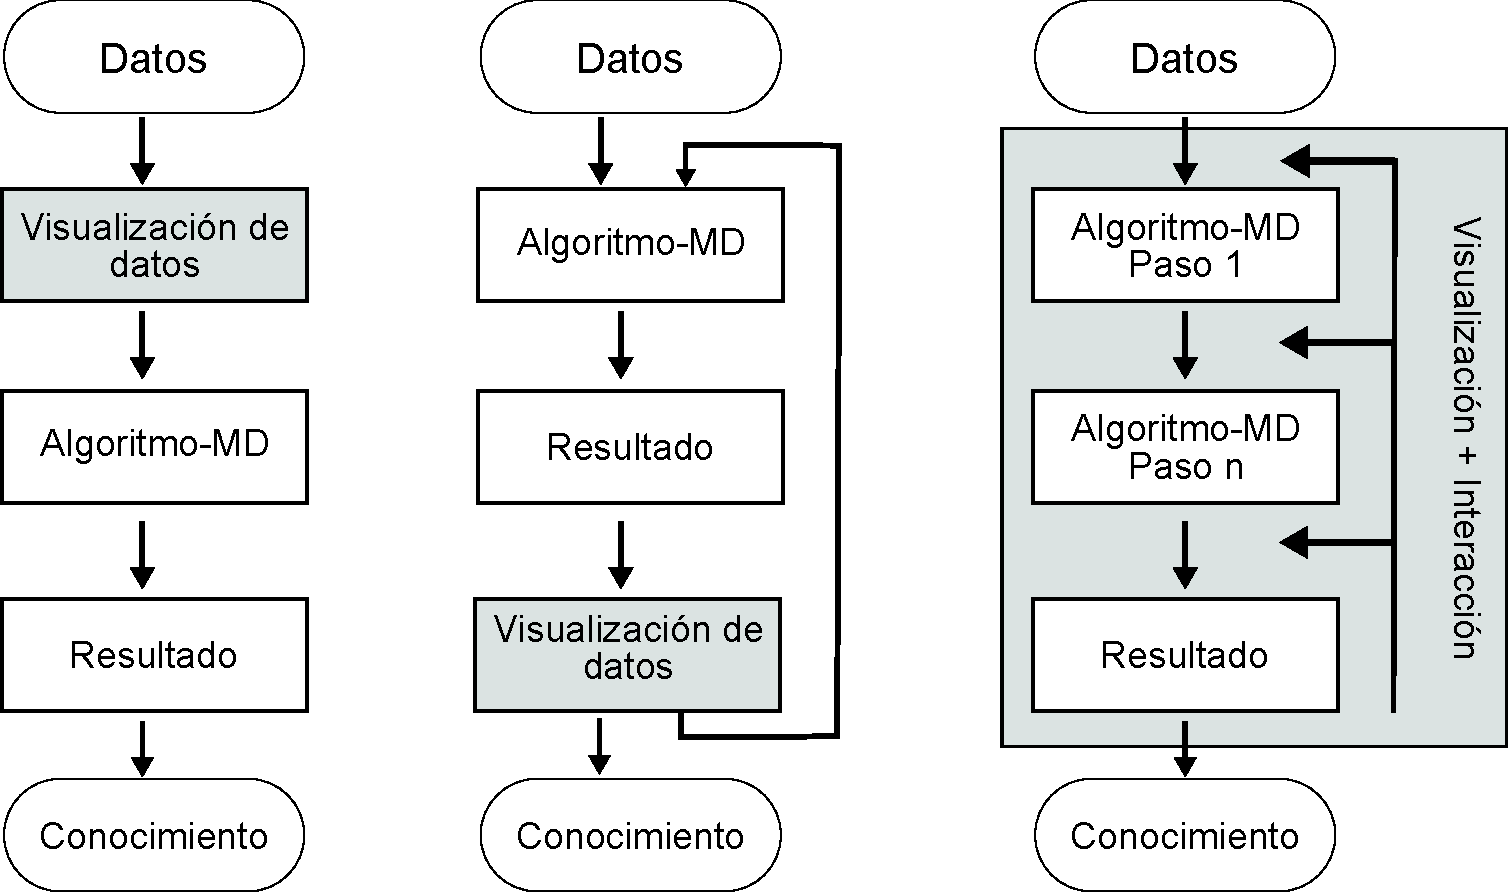
\includegraphics[width=\columnwidth]{figs/VDM.pdf}%
\caption{Vista general de los diferentes enfoques de la integración de los humanos en el proceso de exploración de datos.}%
\label{fig:VDM}%
\end{figure}

\section{Visualización de Información}
La visualización de información \cite{card1999readings} es el uso de representaciones visuales e interactivas de datos para amplificar la cognición. Esto significa que los datos son transformados en una imagen. La imagen puede ser cambiado por los usuarios a media que se vaya trabajando con él. Esta interacción es importante, ya que permite una constante redefinición de objetivos cuando una nueva visión de los datos se han obtenido.
Esta área esta ampliando su espectro debido al desarrollo de la visualización en computadoras en tiempo real. Este medio es promisorio porque acrecienta los recursos del humano en la forma de procesamiento perceptual, permite reducir el tiempo de búsqueda de información, permite mejorar el reconocimiento de patrones, permite el uso de  inferencia y monitoreo perceptual en un medio manipulable e interactivo.
Dentro de las subáreas fundamentales se encuentran la visualización de datos multidimensionales, el cual estudiaremos por la importancia dentro del desarrollo del presente trabajo.
\section{Visualización de Datos Multidimensionales}
		\subsection{Proyecciones Multidimensionales}
		\subsection{Métricas de medición de calidad de una proyección}
		\subsection{Técnicas de visualización Radial}
		\subsection{Radviz}
		\subsection{Star Coordinates}
\section{Consideraciones Finales}
 %Inserta el capítulo 2
\chapter{Nombre del Capítulo}

Cada capítulo deberá contener una breve introducción que describe en forma rápida el contenido del
mismo. En este capítulo va el marco teórico. (pueden ser dos capítulos de marco teórico)

\section{Sección 1 del Capítulo}

Un capítulo puede contener n secciones. La referencia bibliográfica se hace de la siguiente manera:
\cite{Mateos00}

\subsection{Sub Sección}

Una sección puede contener n sub secciones.\cite{Galante01}

\subsubsection{Sub sub sección}

Una sub sección puede contener n sub sub secciones.
\section{Consideraciones Finales}

Cada capítulo excepto el primero debe contener al finalizarlo una sección de consideraciones que enlacen
el presente capítulo con el siguiente.
 %Inserta el capítulo 3
\chapter{iStar}

\section{Propuesta}

\subsection{Pipeline y Framework}

\section{Clusterización de atributos}
	\subsection{Basado PCA}
	
	\subsection{Basado en la Varianza}
	
	\subsection{Basado en Centroides}

\section{Reordenamiento}

	\subsection{Basado en Métricas}
	
	\subsection{Basado en Algoritmos Genéticos}

\section{Operaciones Interactivas}

	
	\begin{itemize}
		\item Escala
		
	\item Rotación

	\item Unión
	
	\item Separación
	
	\item Eliminación
	
	\item Re-Inserción
	
	\item Posicionamiento
	
	\item Node Preview
	
	\item Node Explorer
	
	\item Visualizador de calidad
\end{itemize}

 %Inserta el capítulo 4
\chapter{Pruebas y Resultados}
 %Inserta el capítulo 4
\chapter{Conclusiones y Trabajos Futuros}\label{chap:conclusiones}

Las conclusiones de la tesis son una parte muy importante y tiene las siguientes partes.

En primer lugar debes escribir las conclusiones generales de tu trabajo. evita escribirlas en forma de viñetas. Simplemente utiliza texto continuo.

\section{Limitaciones}
La segunda  parte de este capítulo corresponde a las limitaciones que tiene la propuesta. Esta seccion es muy importante para que los siguientes estudiantes que hagan algo en esta línea no cometan los mismos errores y tu tesis sea un buen peldaño para avanzar más rápido.

\section{Recomendaciones}
En esta sección el tesista debe reflejar que la tesis ha permitido adquirir nuevos conocimientos que podrían servir para guiar otros trabajos en el futuro.

\section{Trabajos futuros}
En base a los puntos anteriores es recomendable que tu tesis también sugiera trabajos futuros. Esta sección es esecialmente útil para otras ideas de tesis.

Todo este capítulo no debe ser más de 4 páginas. %Inserta el capítulo 5

%%%%%%%%%%%%%%%%%%%%%%%%%%%%%%%%%%%%%%%%%%%%%%%%%%%%%%%%%%%%%%%%%%%%%%

\bibliographystyle{apalike}
\bibliography{Bibliog}
\addcontentsline{toc}{chapter}{Bibliografía}

\end{document}
